\documentclass[12pt,letterpaper,noanswers]{exam}
\usepackage[usenames,dvipsnames,svgnames,table]{xcolor}
\usepackage[margin=0.9in]{geometry}
\renewcommand{\familydefault}{\sfdefault}
\usepackage{multicol}
\pagestyle{head}
\header{AM 111 Class 08}{}{Solving equations, p.\thepage}
\runningheadrule
\headrule
\usepackage{siunitx}
\usepackage{graphicx} % more modern
\usepackage{amsmath} 
\usepackage{amssymb} 
\usepackage{hyperref}
\usepackage{tcolorbox}
\usepackage{enumitem}
\def\mbf{\mathbf}
\newcommand{\vc}[1]{\boldsymbol{#1}}
\DeclareMathOperator*{\argmin}{arg\,min} % thin space, limits underneath in displays


\begin{document}
 \pdfpageheight 11in 
  \pdfpagewidth 8.5in

\noindent 

\section*{Preliminaries}

\begin{itemize}
\itemsep0pt
\item Problem set 03 is due on Friday at noon.
\item Problem set 03 includes some ``time permitting'' problems.  If your total time spent on the problem set reaches 8 hours in the week then you are encouraged to skip problems.  If you are not in that situation, you are expected to complete the problems.
\item There will be a skill check in class during Class 09.  The problem info is below.
\item Find all OH on Canvas.
\end{itemize}



\noindent\textbf{Big picture}

Today: Algorithms for approximating solutions to nonlinear equations.

\vspace{0.2cm}
\hrule
\vspace{0.2cm}

\noindent \textbf{Skill check practice}
\begin{questions}
\item For the plot below and the two points indicated, draw the secant line and mark the location of the new approximation of the root, $x_2$.

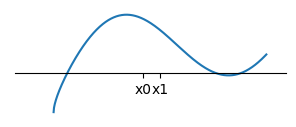
\includegraphics[width=0.6\textwidth]{img/Quiz01secant.png}

\end{questions}


\vspace{0.2cm}
\hrule
\vspace{0.2cm}

\noindent \textbf{Skill check solution}
\begin{questions}
\item Draw a line through $(x_0,f(x_0))$ and $(x_1, f(x_1))$.  That line intersects the $x$-axis at $x_2$.

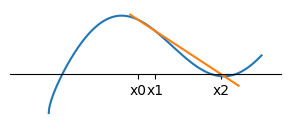
\includegraphics[width=0.6\textwidth]{img/Quiz01secant-soln.png}

\end{questions}
\vspace{0.2cm}
\hrule
\vspace{0.2cm}

\noindent\textbf{Teams}
1. Sara, Ada, Brooke

2. Emma, Trey

3. Kinara, Kyumin

4. Isha, Davin

\section*{Newton's method}

\begin{enumerate}
\item Let $x^*$ be a solution of $f(x) = 0$.  Show that $x^*$ is a fixed point of $x_{k+1} = g(x_k)$ where $g(x) = x - \dfrac{f(x)}{f'(x)}$ (Newton's method).
\vspace{1in}
    \item (Sauer \S1.4 1a) Apply two steps of Newton's method with initial guess $x_0 = 0$ for $f(x) = x^3+x-2$
    \vspace{1in}

        \item For each of the following problems, identify $f(x)$ so that Newton's method can be used.
    \begin{parts}
        \item $x^3 = 25$
        \item $\sin x = 6x + 5$
        \item The amount of pressure, $p$, needed to sink a circular plate of radius $r$ a distance $d$ into soft soil is approximated by $p = x e^{x r} + x r$.   The constant $x$ depends on $d$.  A plate of radius $0.1$ m requires a pressure of $100$ N/m$^2$ to sink $1$ m
    \end{parts}
\vspace{1in}

\item $\dfrac{\left\vert e_{i+1} \right\vert}{\left\vert e_{i} \right\vert} = \dfrac{\left\vert x_{i+1}-x^*\right\vert}{\left\vert \Delta x_i \right\vert} = \dfrac{\left\vert g(x_{i}) -x^*\right\vert}{\left\vert \Delta x_i \right\vert} \approx \dfrac{\left\vert g(x^*) + \Delta x_i g'(x^*) -x^*\right\vert}{\left\vert \Delta x_i \right\vert} = \dfrac{\left\vert  \Delta x_i g'(x^*) \right\vert}{\left\vert \Delta x_i \right\vert} = \left\vert g'(x^*) \right\vert$.

    Find $g'(x^*)$ for Newton's method.  Is this method superlinear, linear, or sublinear?
    \end{enumerate}
    \vspace{1in}

        Newton's method converges quadratically: $\lim\limits_{i\rightarrow\infty} \dfrac{\vert e_{i+1}\vert }{\vert e_i\vert^2 } = \dfrac{\vert f''(x^*)\vert}{2\vert f'(x^*)\vert} = C < \infty$
 
\subsection*{Order of convergence}

   \begin{enumerate}[resume]
    \item (Heath \S 5.4) Match the error sequence with convergence information.
    
    \begin{enumerate}
    \item quadratic convergence
    \item linear convergence with $C = 10^{-1}$
    \item linear convergence with $C = 10^{-2}$
    \item superlinear but slower than quadratic
    \end{enumerate}
    
    \begin{enumerate}
    \item[(i)] $10^{-2},10^{-4},10^{-6},10^{-8},...$
    \item[(ii)] $10^{-2},10^{-4},10^{-8},10^{-16},...$
    \item[(iii)] $10^{-2},10^{-4},10^{-7},10^{-12},...$
    \item[(iv)] $10^{-2},10^{-3},10^{-4},10^{-5},...$
    \end{enumerate}
\end{enumerate}


\begin{enumerate}[resume]
\item For sufficiently large $k$, $\dfrac{\vert e_{k+1}\vert}{\vert e_k\vert^r} \approx C$.
\begin{parts}
\item $\vert e_{k+1}\vert\approx C\vert e_k\vert^r$.  Write a similar expression for $\vert  e_{k+2}\vert $.
\vspace{0.5in}

\item Use the ratio of your expressions to show that $\log \left\vert\dfrac{e_{k+2}}{e_{k+1}}\right\vert \approx r \log \left\vert\dfrac{e_{k+1}}{e_{k}}\right\vert$
\vspace{1in}

\item Rearrange to produce an expression that approximates $r$.
\end{parts}
\end{enumerate}


\subsection*{Secant method}

\subsection*{Summary}
\begin{tabular}{p{0.3\linewidth} p{0.3\linewidth} p{0.3\linewidth}}
bisection & Newton's & secant \\
\hline
always converges & may not converge & may not converge\\
sign of $f$  & needs $f$ and $f'$ & just needs $f$ \\
$f$ continuous & $f$ differentiable & $f$ continuous\\
linear convergence & quadratic convergence & superlinear ($<$ quadratic) \\
needs initial interval & one initial value& two initial values\\
no higher-dim'l version & higher dim'l version & \\
\end{tabular}

\begin{enumerate}[resume]
\item (Health \S5 5.24)

List one advantage and one disadvantage of the secant method compared with Newton's method for solving a nonlinear equation in one dimension.
\vspace{0.5in}

\item (Heath \S5 5.32) 

Think about how you might combine the idea of  a bracket around the solution from the bisection method with the secant method so that the method will still converge even if it starts far from a root.

\emph{This is called a safeguarded method}

\vspace{0.5in}
\end{enumerate}

\section*{Newton's method in higher dimensions}




\begin{enumerate}[resume]
\item Consider the problem of finding $(x,y)$ such that $\sin(x) = e^y$ and $x^2 + y^2 = 8$.

Find $\mathbf{f}$ and $D\mathbf{f}$ for solving this system via Newton's method.
\end{enumerate}



\eject
\section*{Numerical Case Study: Root finding methods}

We are going to use bisection, Newton's method, and the secant method.  Find the code on Canvas.  Investigate four functions:
\begin{enumerate}
\item[f1] $f_1(x) = x^2 - x - 6$ (roots -2,3)
\item[f2] $f_2(x) = x^3 - x^2$ (roots 0,1)
\item[f3] $f_3(x) = x^3 - 2x^2 + \frac{4x}{3} - \frac{8}{27}$ (root 2/3)
\item[f4] $f_4(x) = x - 2^{-x}$
\end{enumerate}
\begin{enumerate}[resume=classQ]
    \item Download the file from github: \url{https://github.com/sarah1123/ScientificComputing-APMTH111/blob/main/2023Fall/Class/08-rootfinding.ipynb}.
    \item Check that the functions and derivatives defined in the Jupyter Notebook correspond to the functions above.
\end{enumerate}



\subsection*{Bisection Method}

\noindent
Try the bisection method. The code includes parameters that you might want to change while going through the tasks below, and generates a figure of the estimate of the order $r$ of the method.  Note that $[a,b]$ is your initial interval for estimating the root in this code. 

\begin{enumerate}[resume=classQ]
\item Find starting intervals that lead to finding the roots of each function.

\vfill

\item Is there an issue with a root of $f2$? Why?

\vfill

%\item Save a screenshot of your answers on this page and a plot of your estimate of $\alpha$ for $f1$.

%\vfill

\end{enumerate}










\subsection*{Newton's Method}

\noindent
Now try Newton's method.  Note that $x$ is your initial estimate for the root in this code.

\begin{enumerate}[resume=classQ]
\item Find initial guesses that converge to each root for each function, as well as initial guesses that don't converge for each function.

\vfill

\item For $f1$, do you see a doubling of zeros in the accuracy? Look at the printout of the estimate of the root.

\vfill

\pagebreak
\item For the $f2$ double root at zero, the estimate for $r$ should be around 1.  Newton's method only converged quadratically for simple roots.  To increase the convergence at a double root, observe that $f^{1/2}$ has a simple root.  Find $\dfrac{\sqrt{f}}{\frac{d}{dx}\sqrt{f}}$.  This leads to a modified Newton's method: $x_{k+1} = x_k - 2\dfrac{f(x_k)}{f'(x_k)}$.  

\emph{Another option for a double root is to observe that $g(x) = \dfrac{f(x)}{f'(x)}$ will have a single root at the same location.}

\vfill

\item Estimate $r$ for $f2$ using modified Newton's method.


\end{enumerate}








%\pagebreak
\section*{Secant Method}

\noindent
Next work with the secant method.  Note that $xOld$ and $x$ are your two initial estimates for the root in this code.

\begin{enumerate}[resume=classQ]
\item Find initial guesses that converge to each root for each function.

\vfill

\item Find initial guesses that don't converge to a root for each function.

\vfill

\item Make a plot of your estimate of $r$ for $f4$.

\vfill

\end{enumerate}

\end{document}